\chapter{Theory} \label{CH:theory}
%\textbf{What is your thought process in how to solve this problem??\\
%How do you propose solving this problem?\\
%What is a dual grid?\\
%What is a height function?\\
%How does it work?\\
%Why do we choose to use a HFM?\\
%Shortcomings of HFM's?\\
%On this dual grid, why do we need a fine velocity?}\\
Computational solutions for fluid flow rely on several fundamental ideas surrounding how fluids are simulated. The following section is an attempt to summarize several of these methods and lay the necessary framework for understanding the subsequent method, which is the primary focus of this work. Each of the methods discussed are present within NGA, the computational platform used in this research. Additionally, while these methods are prevalent in the CFD community, they are not the only options available. The interested reader is directed to \ref{TRYG} for a more comprehensive assessment.   

\subsection{The Navier-Stokes Equations}
They exist, here they are....
\hl{consider discussion}

\subsection{Computational Platform}
The proposed curvature estimation method exists as a module within a larger computational framework. While this scheme can be incorporated into any number of solvers, the platform used for this work was NGA~\cite{NGA1,NGA2}.  NGA solves low-Mach number, variable density formulations of mass and momentum conservation laws
\begin{align}
\frac{\partial \rho_\phi}{\partial t} +& \nabla \cdot \left(\rho_\phi\bm{u}_\phi\right) = 0\mbox{ \quad and}\\
\frac{\partial \rho_\phi \bm{u}_\phi}{\partial t} +& \nabla \cdot \left(\rho_\phi\bm{u}_\phi\otimes\bm{u}_\phi\right) = -\nabla p_\phi + \nabla\cdot\left(\mu_\phi\left[\nabla\bm{u}_\phi+\nabla\bm{u}_\phi^\mathsf{T}\right]\right)+\rho_\phi\bm{g}
\end{align}
where
$\rho_\phi$ is the density,
$\bm{u}_\phi=[u,v,w]_\phi$ is the velocity field vector,
$t$ is time,
$p_\phi$ is the hydrodynamic pressure,
$\mu_\phi$ is the dynamic viscosity, and
$\bm{g}$ is the gravitational acceleration.
The subscript
$\phi$ indicates the phase and takes values of $\phi=g$ or
$\phi=l$ in the gas or liquid phase, respectively.

These equations have been written in both the gas and liquid phases and are connected through jump conditions at the phase interface.
For example, the jumps in density and viscosity at the interface
$\Gamma$ are written as 
\begin{align}
[\rho]_\Gamma&%
=\rho_l-\rho_g\mbox{\quad and}\\
[\mu]_\Gamma&%
=\mu_l-\mu_g.
\end{align}
In the absence of a phase change, the velocity field is continuous, \ie, 
\begin{equation}
[\bm{u}]_\Gamma=0.
\end{equation}
The pressure is discontinuous due to contributions from surface tension and the normal component of the viscous stress, \ie,
\begin{equation}
[p]_\Gamma=\sigma\kappa+ 2\left[\mu\right]_\Gamma\bm{n}^\mathsf{T}\cdot\nabla\bm{u}\cdot\bm{n},
\end{equation}
where
$\sigma$ is the surface tension coefficient and
$\kappa$ is the interface curvature. This is the curvature that is computed with the height function method.

These equations are discretized using a Cartesian mesh with pressure and other scalars located at cell centers and velocity components located at cell faces. Time is discretized using an iterative second order Crank-Nicolson formulation with a semi-implicit correction on each subiteration~\cite{choi}. The interface is represented with a geometric volume-of-fluid (VoF) method~\cite{Owkes2017,Owkes2014}. The NGA code is highly parallelized, allowing for scalable simulations and fast run times and has been applied to many atomization applications~\cite{OwkesAIAA,Desjardins2013,sheehy}.

\subsection{Mesh Generation}
In Numerical analysis, the grid or mesh, often refers to the manner in which a domain being simulated is subdivided into smaller sections and points. Traditionally these points are denoted using an i,j scheme and neighboring points will be referenced from an initial point as seen in Figure \ref{fig:ijGrid}. This method is extended similarly in the z-direction for 3D applications~\cite{MIT}.  

	\begin{figure}[htbp]
		\centering
		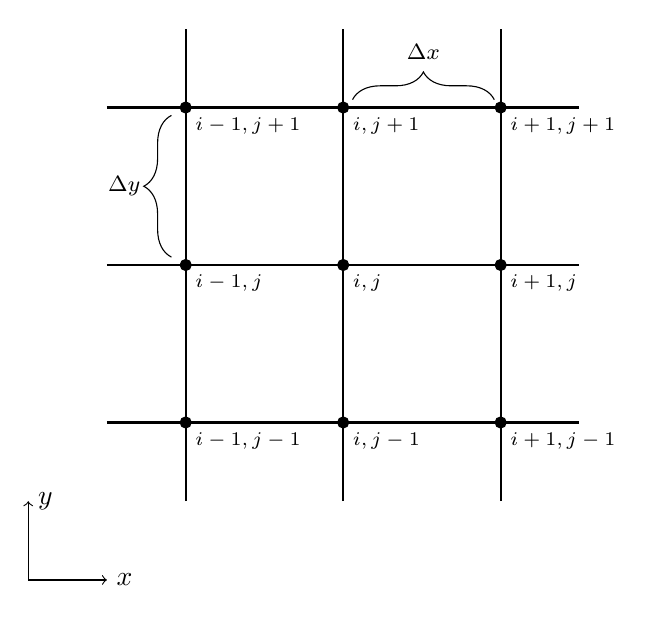
\begin{tikzpicture}[scale=2.0]
		% Mesh
		\draw [black,thick,step=1.0] (0.5 , 0.5) grid (3.5,3.5); 
		% i's and j's
			\node[below right] at (1,1) {\scriptsize{$i-1,j-1$}};
			\node[below right] at (1,2) {\scriptsize{$i-1,j$}};
			\node[below right] at (1,3) {\scriptsize{$i-1,j+1$}};
			\node[below right] at (2,1) {\scriptsize{$i,j-1$}};
			\node[below right] at (2,2) {\scriptsize{$i,j$}};
			\node[below right] at (2,3) {\scriptsize{$i,j+1$}};
			\node[below right] at (3,1) {\scriptsize{$i+1,j-1$}};
			\node[below right] at (3,2) {\scriptsize{$i+1,j$}};
			\node[below right] at (3,3) {\scriptsize{$i+1,j+1$}};
		%Node Circles
			\draw [fill] (2,2) circle [radius=0.035];
			\draw [fill] (1,2) circle [radius=0.035];
			\draw [fill] (3,2) circle [radius=0.035];
			\draw [fill] (2,1) circle [radius=0.035];
			\draw [fill] (2,3) circle [radius=0.035];	
			\draw [fill] (1,1) circle [radius=0.035];
			\draw [fill] (1,3) circle [radius=0.035];
			\draw [fill] (3,1) circle [radius=0.035];
			\draw [fill] (3,3) circle [radius=0.035];		
		%Axes
			\draw [arrows=->] (0,0) -- node[pos=1,right] {$\bm{x}$} (0.5,0);
			\draw [arrows=->] (0,0) -- node[pos=1,right] {$\bm{y}$} (0,0.5);
		%Dx Dy
			\draw [decorate,decoration={brace,amplitude=10pt},xshift=-4pt,yshift=0pt] (1.05,2.05) -- (1.05,2.95) node [black,midway,xshift=-0.6cm] {\footnotesize $\Delta y$};
			\draw [decorate,decoration={brace,amplitude=10pt},xshift=-4pt,yshift=0pt] (2.2,3.05) -- (3.1,3.05) node [black,midway,yshift=0.6cm] {\footnotesize $\Delta x$};
		\end{tikzpicture}
		\caption{Typical notation of structured grid cells.}
		\label{fig:ijGrid}
	\end{figure}

\paragraph{} The type of grid used can be classified as being in one of two categories, structured or unstructured~\cite{anderson}. The choice of whether to use a structured or unstructured grid should be considered on a case by case basis. However, there are some important characteristics of each that are important to recognize prior to implementation. A structured grid in 2D can be thought of a series of quadrilateral elements (bricks) placed side by side in a uniform fashion~\cite{MIT}. Here, neighboring elements are referenced by adding or subtracting from the base cell indices~\cite{anderson}. Figure \ref{fig:Simple Grid} is an example of a structured grid. An unstructured grid does not retain uniformity and is normally (although, not always) comprised of triangular elements~\cite{tu}. To reference neighboring cells in an unstructured grid, storage of cell-to-cell pointers are required~\cite{MIT}. Unstructured grids normally require a greater amount of memory storage and can result in slower computation times than that of a structured grid~\cite{magoules}. A simplified example of an unstructured grid can be referenced in Figure \ref{fig:Unstructured Grid}. The NGA code, which is this focus of this research, uses a structured grid approach for simplicity and computational efficiency. However, it should be noted that unstructured grids are increasing in popularity as the accuracy obtained from modeling complex flow geometry may be higher than that of a structured grid~\cite{Hirt1981}. 

\begin{figure}[htbp]
	\centering
	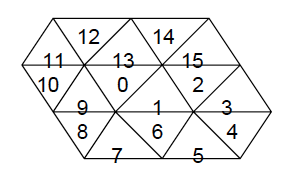
\includegraphics[width=2.5in]{figs/unstruc}
	\caption{Simple Unstructured Grid \cite{MIT}}
	\label{fig:Unstructured Grid}
\end{figure}

\subsection{Volume of Fluid Formulation}
In order to accurately predict the behavior of a multiphase system, the location of the interface of the two fluids must be determined. One method for completing this is known as the Volume of Fluid (VOF) method. This method was first introduced by Hirt \& Nichols (1981) and has been expanded upon by several others~\cite{Hirt1981,1,2,3,4}. The defining contribution of the VOF method proposed by Hirt \& Nichols is the introduction of a scalar marker function assigned to each mesh cell which is indicative of the volume of a given fluid within that cell~\cite{Hirt1981}. This allows for interface to be tracked by the value of the marker cell in surrounding cells. For example, if $VOF = 1.0$ indicates a region of liquid and $VOF = 0.0$ indicates a region of gas, then a cell with a value $0.0 \leq VOF \leq 1.0$ indicates a cell which contains interface. It is important to recognize that volume of a fluid may only be advected into a new cell once the current cell is full~\cite{TRYG}. A one-dimensional example of this advection can be seen in Figure \ref{fig:1Dadvect}.

\begin{figure}[htbp]
	\centering
	\begin{tikzpicture}[scale=3.0]
	% Mesh
	\draw [lightblue,fill=lightblue] (0.0,0.0) -- (1.25,0.0) -- (1.25,1.0) -- (0.0,1.0) -- cycle;
	\draw [black,thick,step=1.0] (0.0 , 0.0) grid (3.0,1.0); 
	%Velocity
	\draw [arrows=->, thick] (1.25,0.5) -- node[pos=1,right] {$u$} (1.5,0.5);
	%Labels
	\node[] at (0.5,-0.15) {\scriptsize{$VOF(i-1)=1.0$}};
	\node[] at (1.5,-0.15) {\scriptsize{$VOF(i)=0.25$}};
	\node[] at (2.5,-0.15) {\scriptsize{$VOF(i+1)=0.0$}};
	\end{tikzpicture}
	\caption{Advection of a one-dimensional fluid interface}
	\label{fig:1Dadvect}
\end{figure}

The advection procedure for a VOF method is completed in two primary steps. First, the interface needs to be geometrically constructed. Second, the constructed interface is advected with the current velocity field\cite{TRYG}. Figure \ref{fig:1Dadvect} depicts one-dimensional interface advection. In this case, geometric reconstruction is accomplished with a single vertical line. Adoption of this method is straightforward. As simulations increase to two or three dimensional analysis however, this problem quickly becomes non-trivial. Early attempts to resolve this difficulty include the Simple Line Interface Calculation (SLIC) method of Noh and Woodward (1976)\cite{NohWoodward}. Here, the reconstructed interface is made up of lines which align parallel to the mesh in both \textit{x} and \textit{y} directions.      
     
\begin{figure}[htbp]
	\centering
	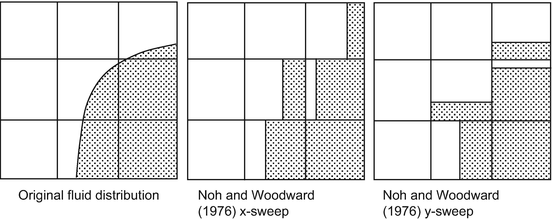
\includegraphics[width=0.7\textwidth]{figs/SLIC.png}
	\caption{Simple Line Interface Calculation of Noh and Woodward adapted from \cite{SLICfig}}
	\label{fig:SLIC}
\end{figure}

Improvement to the SLIC method was presented by Youngs (1982)  known as the Piecewise Linear Interface Calculation (PLIC)~\cite{youngs}. In the PLIC method, instead of aligning interfacial reconstruction lines with the mesh, a line (2D) or plane (3D) is oriented with a normal vector which is evaluated from the volume fraction gradient~\cite{yeoh}. An example of PLIC can be seen in Figure \ref{fig:PLIC}. This method is a popular geometric reconstruction scheme still today and is used in NGA for this research.

\begin{figure}[htbp]
	\centering
	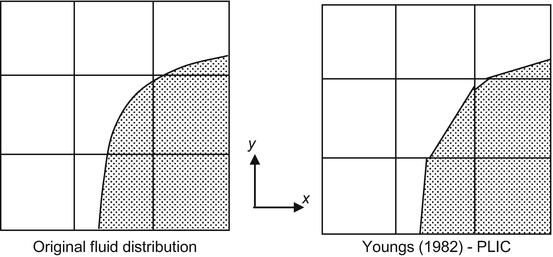
\includegraphics[width=0.5\textwidth]{figs/PLIC.png}
	\caption{Piecewise Linear Interface Calculation of Youngs adapted from \cite{yeoh}}
	\label{fig:PLIC}
\end{figure}

\subsection{Rudman Dual Grid Formulation}
Solution of the incompressible Navier-Stokes equations traditionally occurs on whats known as a staggered grid. On a staggered grid, pressure is typically stored at cell centers and velocity components are stored at cell faces~\cite{TRYG}. Building from the structured grid example given in Figure \ref{fig:ijGrid}, this implementation is illustrated in Figure \ref{fig:StagGrid}. 

 \begin{figure}[h!]
 	\centering
 	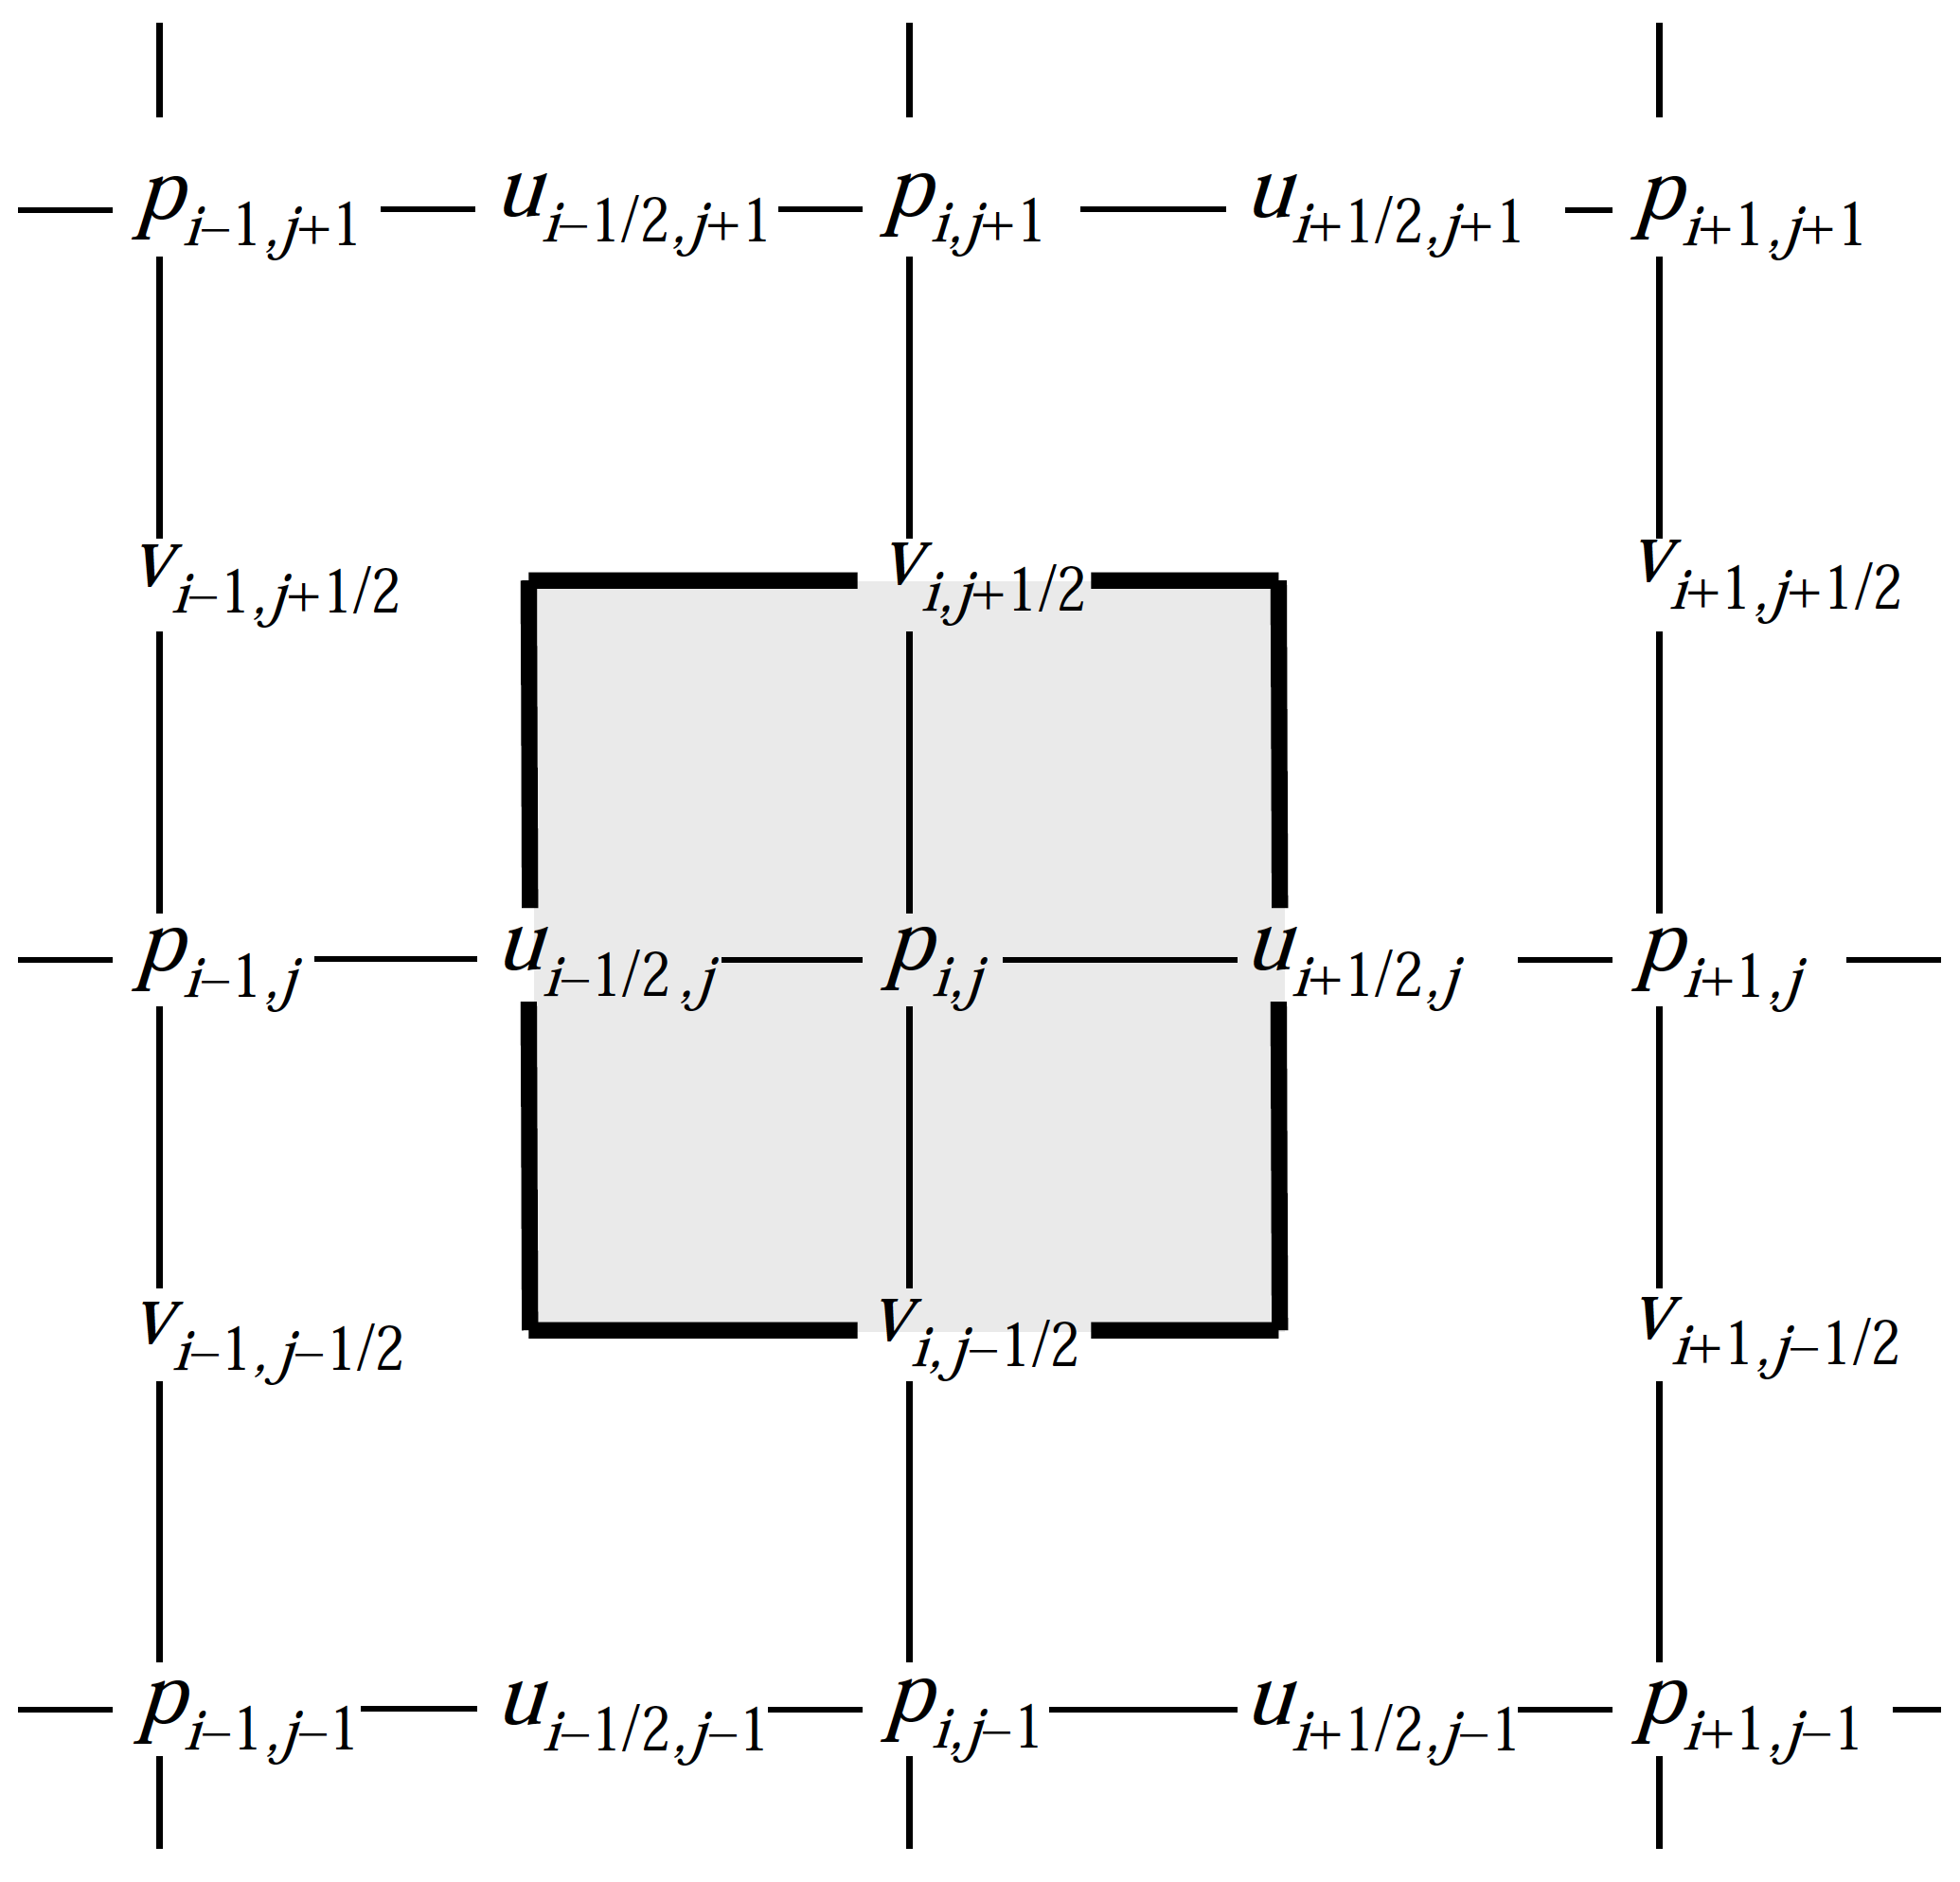
\includegraphics[width=2.5in]{figs/StaggeredGrid}
 	\caption{Typical staggered grid, adopted from \cite{TRYG}.}
 	\label{fig:StagGrid}
 \end{figure}

\noindent This approach was first introduced by Harlow and Welch (1965) and is now considered the standard approach in structured mesh CFD applications today \cite{HARLOW1965}. For incompressible flows, staggered grids offer the advantage of tightly coupling fluid property variables as well as eliminating pressure-velocity checkerboarding~\cite{rudman}. The Rudman Dual grid approach, first presented by Rudman (1998), is a technique developed for high density ratio, multiphase flows, which accurately conserves both mass and momentum. This is achieved by calculating momentum-flux values on a twice as fine mesh near the fluid interface as illustrated in Figure \ref{fig:rudmesh}~\cite{Rudman}. The Rudman Dual mesh is incorporated into NGA and is essential to the formulation of the method presented in this research.

\begin{figure}[htbp]
	\centering
	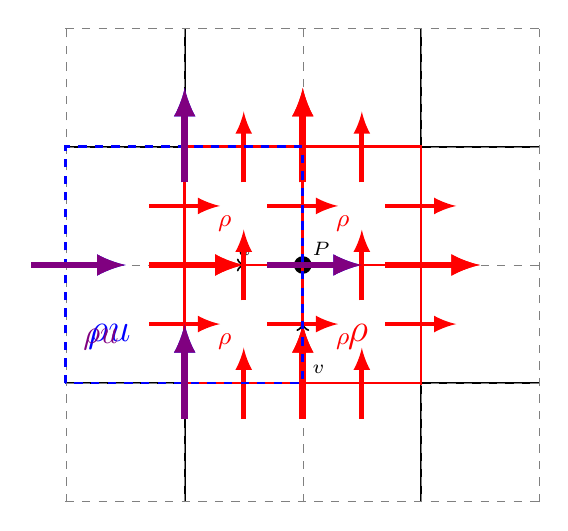
\begin{tikzpicture}[scale=3]
	% Mesh
	\draw [black,thick,step=1.0] (1.5 , 1.5) grid (3.5,3.5);
	\draw [dashed,step=0.5, help lines] (1.495 ,1.495) grid (3.5,3.5);
	%Cell centered dots
	\draw [fill] (2.5,2.5) circle [radius=0.035];
		% Pressure nodes
		\node [above right] at (2.5,2.5) {\scriptsize{$P$}};
%	% U Velocity Arrows
	\draw [arrows=->,line width=0.75] (2.0,2.5) -- (2.25,2.5);

		\node [above] at (2.25,2.5) {\scriptsize{$u$}};
		\draw [arrows=->,line width=0.75] (2.5,2.0) -- (2.5,2.25);
		\node [above right] at (2.5,2.0) {\scriptsize{$v$}};
	
%	% Overlay density RED
	\draw[red,line width=1.0] (2.0,2.0) rectangle (3.0,3.0);
		\node [red,above right] at (2.65,2.1) {\Large{$\rho$}};
		%Vertical arrows
		\draw[red,arrows=-latex,line width=2.5] (2.5,1.85) -- (2.5,2.25);
		\draw[red,arrows=-latex,line width=2.5] (2.5,2.85) -- (2.5,3.25);
		%Horizontal arrows
		\draw[red,arrows=-latex,line width=2.5] (1.85,2.5) -- (2.25,2.5);
		\draw[red,arrows=-latex,line width=2.5] (2.85,2.5) -- (3.25,2.5);
%	% Overlay momentum BLUE
	\draw[blue,dashed,line width=1.0] (1.495,2.0) rectangle (2.5,3.0);
		\node [blue,above right] at (1.55,2.1) {\Large{$\rho u$}};
		%Vertical arrows
		\draw[blue,arrows=-latex,line width=2.5] (2.0,1.85) -- (2.0,2.25);
		\draw[blue,arrows=-latex,line width=2.5] (2.0,2.85) -- (2.0,3.25);
		%Horizontal arrows
		\draw[blue,arrows=-latex,line width=2.5] (1.35,2.5) -- (1.75,2.5);
		\draw[blue,arrows=-latex,line width=2.5] (2.35,2.5) -- (2.75,2.5);
		% Overlay density arrows again RED
		%Vertical arrows
		\draw[red,arrows=-latex,line width=2.5] (2.5,1.85) -- (2.5,2.25);
		\draw[red,arrows=-latex,line width=2.5] (2.5,2.85) -- (2.5,3.25);
		%Horizontal arrows
		\draw[red,arrows=-latex,line width=2.5] (1.85,2.5) -- (2.25,2.5);
		\draw[red,arrows=-latex,line width=2.5] (2.85,2.5) -- (3.25,2.5);
	% Rudman's Method
	% Overlay density RED
	\draw[red, step= 0.5, line width=1.0] (1.99,1.99) grid (3.0,3.0);
		\node [red,above right] at (2.6,2.1) {\small{$\rho$}};
		\node [red,above right] at (2.6,2.6) {\small{$\rho$}};
		\node [red,above right] at (2.1,2.1) {\small{$\rho$}};
		\node [red,above right] at (2.1,2.6) {\small{$\rho$}};
%		%Vertical arrows
		\draw[red,arrows=-latex,line width=1.75] (2.25,1.85) -- (2.25,2.15);
		\draw[red,arrows=-latex,line width=1.75] (2.25,2.35) -- (2.25,2.65);
		\draw[red,arrows=-latex,line width=1.75] (2.25,2.85) -- (2.25,3.15);
		\draw[red,arrows=-latex,line width=1.75] (2.75,1.85) -- (2.75,2.15);
		\draw[red,arrows=-latex,line width=1.75] (2.75,2.35) -- (2.75,2.65);
		\draw[red,arrows=-latex,line width=1.75] (2.75,2.85) -- (2.75,3.15);
		%Horizontal arrows
		\draw[red,arrows=-latex,line width=1.75] (1.85,2.25) -- (2.15,2.25);
		\draw[red,arrows=-latex,line width=1.75] (2.35,2.25) -- (2.65,2.25);
		\draw[red,arrows=-latex,line width=1.75] (2.85,2.25) -- (3.15,2.25);
		\draw[red,arrows=-latex,line width=1.75] (1.85,2.75) -- (2.15,2.75);
		\draw[red,arrows=-latex,line width=1.75] (2.35,2.75) -- (2.65,2.75);
		\draw[red,arrows=-latex,line width=1.75] (2.85,2.75) -- (3.15,2.75);
	% Overlay momentum BLUE
	    \draw[blue,dashed,line width=1.0] (1.495,2.0) rectangle (2.5,3.0);
		\node [violet,above right] at (1.53,2.1) {\large{$\rho u$}};
		%Vertical arrows
		\draw[violet,arrows=-latex,line width=2.5] (2.0,1.85) -- (2.0,2.25);
		\draw[violet,arrows=-latex,line width=2.5] (2.0,2.85) -- (2.0,3.25);
		%Horizontal arrows
		\draw[violet,arrows=-latex,line width=2.5] (1.35,2.5) -- (1.75,2.5);
		\draw[violet,arrows=-latex,line width=2.5] (2.35,2.5) -- (2.75,2.5);
	\end{tikzpicture}
		\caption{\hl{FIX THIS FIGURE}}
	\label{fig:rudmesh}
\end{figure}

\subsection{Curvature Estimation - Height Function Methods}

Curvature can be discretely described as the reciprocal of radius of a given surface as illustrated in Figure \ref{fig:curv} \cite{MARK2013}. 

 \begin{figure}[htbp]
	\centering
	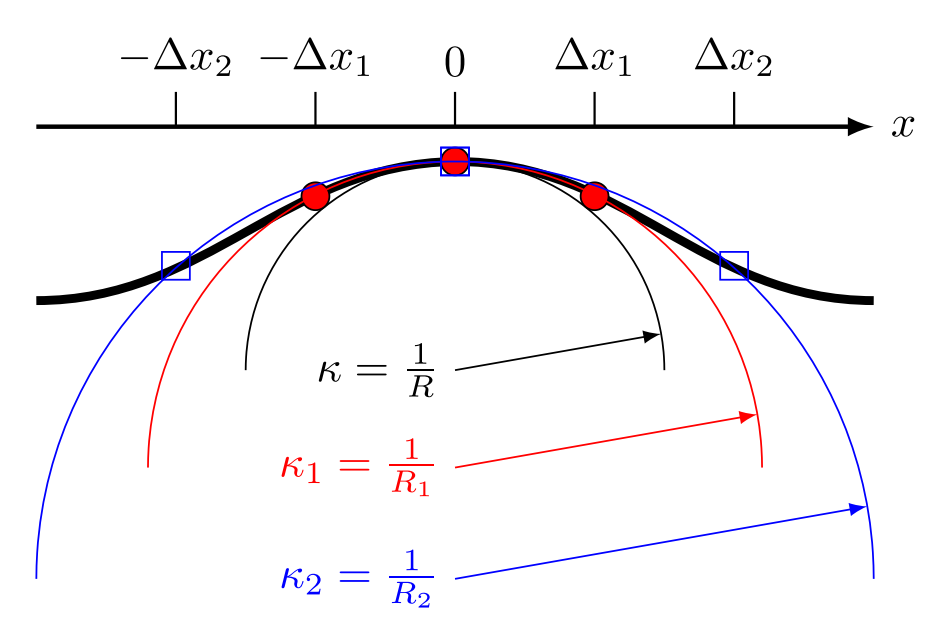
\includegraphics[width=2.5in]{figs/curv}
	\caption{Typical staggered grid, adopted from \cite{TRYG}.}
	\label{fig:curv}
\end{figure}

\noindent Accurate simulations of multiphase flows require an accurate estimation of interface curvature. Figure \ref{fig:surf} illustrates this importance by presenting two atomizing jet simulations. These simulations vary only by their Weber number, which is directly proportional to the surface tension term, and thereby, the curvature at the interface. It is clear that the jet seen in Figure \ref{fig:surf}(b) is experiencing far greater breakup than that seen in Figure \ref{fig:surf}(a). The correct representation of reality is highly dependent on the estimation of curvature made by the numerical model. 

 \begin{figure}[htbp]
	\centering
	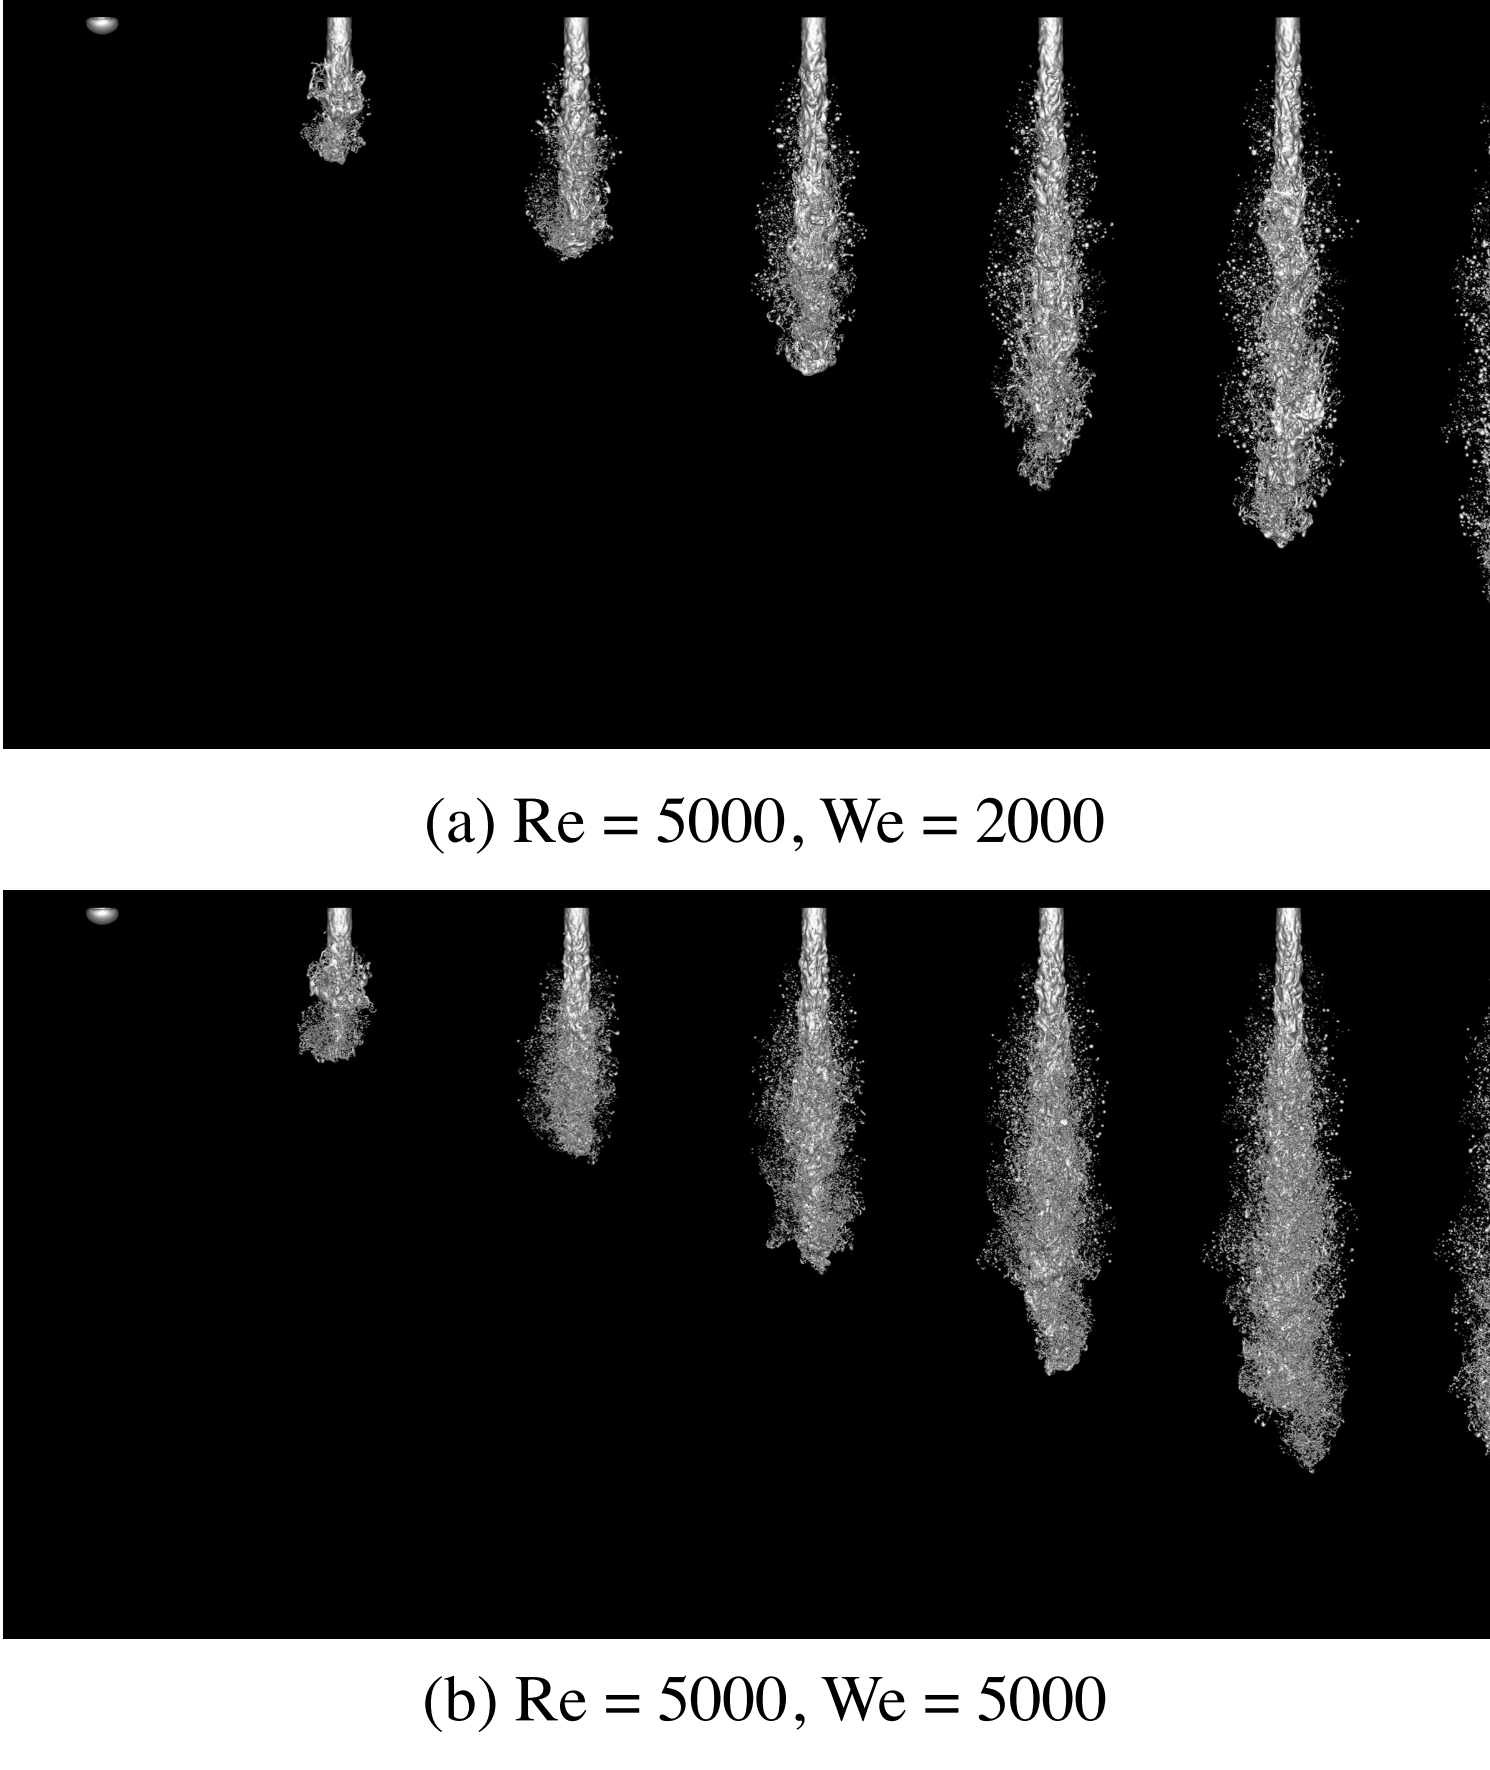
\includegraphics[width=1.5in]{figs/surf}
	\caption{Atomization simulations with varying Weber number, adopted from \cite{Desjardins13}.\hl{figure this spacing out}}
	\label{fig:surf}
\end{figure}

Many techniques exist for calculating values of curvature, some of these include:  level set methods,  height functions, coupled level set volume of fluid (CLSVOF) methods, and others~\cite{1,2,3,4}. The focus of this work specifically, is on modified height function methods.

 \begin{figure}[htbp]
	\centering
	\begin{tikzpicture}[scale=1.15]
		% Mesh
		\draw [step=1.0, help lines] (0.5,0.5) grid (7.5,5.5);
		% Liquid
		\draw [line width=0,fill=lightblue] (0.5,3.5) to[out=20,in=170] (4,4.5) to[out=-10,in=100] (7.0,0.5);
		\draw [lightblue,fill=lightblue] (0.5,3.5) -- (7.0,0.5) -- (0.5,0.5) -- cycle;
		\draw [step=1.0, help lines] (0.5,0.5) grid (7.5,5.5);
		% kappa 1
		\draw [fill] (3.5,4.55) circle [radius=0.1];
		\node [above right] at (3.5,4.55) {$\kappa$};
		\draw [arrows=->,line width=1.0] (2.5,2) -- (2.5,4.35);\node [below] at (2.5,2) {\scriptsize $h_{-1}$};
		\draw [arrows=->,line width=1.0] (3.5,2) -- (3.5,4.55);\node [below] at (3.5,2) {\scriptsize $h_{0}$};
		\draw [arrows=->,line width=1.0] (4.5,2) -- (4.5,4.35);\node [below] at (4.5,2) {\scriptsize $h_{1}$};
		% Triad
		\begin{scope}[shift={(0.5,0.5)}] 
			\draw [arrows=->] (0,0) -- node[pos=1,right] {$\bm{x}$} (0.5,0);
			\draw [arrows=->] (0,0) -- node[pos=1,right] {$\bm{y}$} (0,0.5);
		\end{scope}
	\end{tikzpicture}
	\caption{Traditional height function} 
	\label{fig:hts}
\end{figure}

\noindent Height functions work by integrating volume fractions ($\alpha$) within columns of cells as in equation \ref{eqn:hts} to form heights. A similar approach is taken using widths where an interface is more vertical than horizontal.
 

\begin{equation}
h_{i} = \sum_{i-1}^{i+1} \alpha_{i,j} \Delta y
\label{eqn:hts}
\end{equation}

\noindent Figure \ref{fig:hts} gives an example of heights at a liquid-gas interface. In the simplest execution of a height function, approximation of the curvature ($\kappa$) at the point on the grid is achieved by using a simple finite difference of the heights to approximate first and second derivatives as seen in equations \ref{eqn:1st} and \ref{eqn:2nd} respectively. 

\begin{equation}
H_{x} = \frac{h_{i-1,j}-h_{i+1,j}}{2 \Delta x}
\label{eqn:1st}
\end{equation}
\begin{equation}
H_{xx} = \frac{h_{i+1,j}-2h_{i,j}+h_{i-1,j}}{ \Delta x^2}
\label{eqn:2nd}
\end{equation}

\noindent Finally, curvature is calculated using:
\begin{equation}
\kappa = \frac{-H_{xx}}{(1+H_{x}^{2})^{\frac{3}{2}}}.
\label{eqn:kap}
\end{equation}

\noindent Clearly the above explanation is relevant for two-dimensional flows. Extension to three-dimensional flows is trivial.

Height functions remain a prevalent method for estimating curvature because of their relative ease of implementation. However, several adjustments to the standard model have been proposed. Adjustments include changing the stencil size over which the heights are gathered~\cite{1}, separating the columns from the computational mesh~\cite{2}, combining heights and widths for approximation~\cite{2}, and applying the approach to level sets~\cite{2}(\hl{this sentence is a paraphrase from Mark's 18 JCP consider revising}).


\subsection{Using Height Functions in Conjunction with Rudman Dual Mesh }

When a dual grid is used, the standard height function method fails to capture the dynamics occurring on the fine grid. Left unmitigated, these dynamics can result in fine grid interfacial perturbations, small discontinuities in interface structures. These perturbations can grow uncontrollably and result in non-physical dynamics materializing in simulations. An example of this uncontrolled growth resulting in non-physical dynamics can be seen in Figure~\ref{bad2}. The focus of this research is to develop an extension of the standard height function to include information from the Rudman dual mesh. This method results in consistent mass and momentum transport while also providing accurate interface transport that avoids non-physical dynamics.


\begin{figure}[htbp]
	\centering
		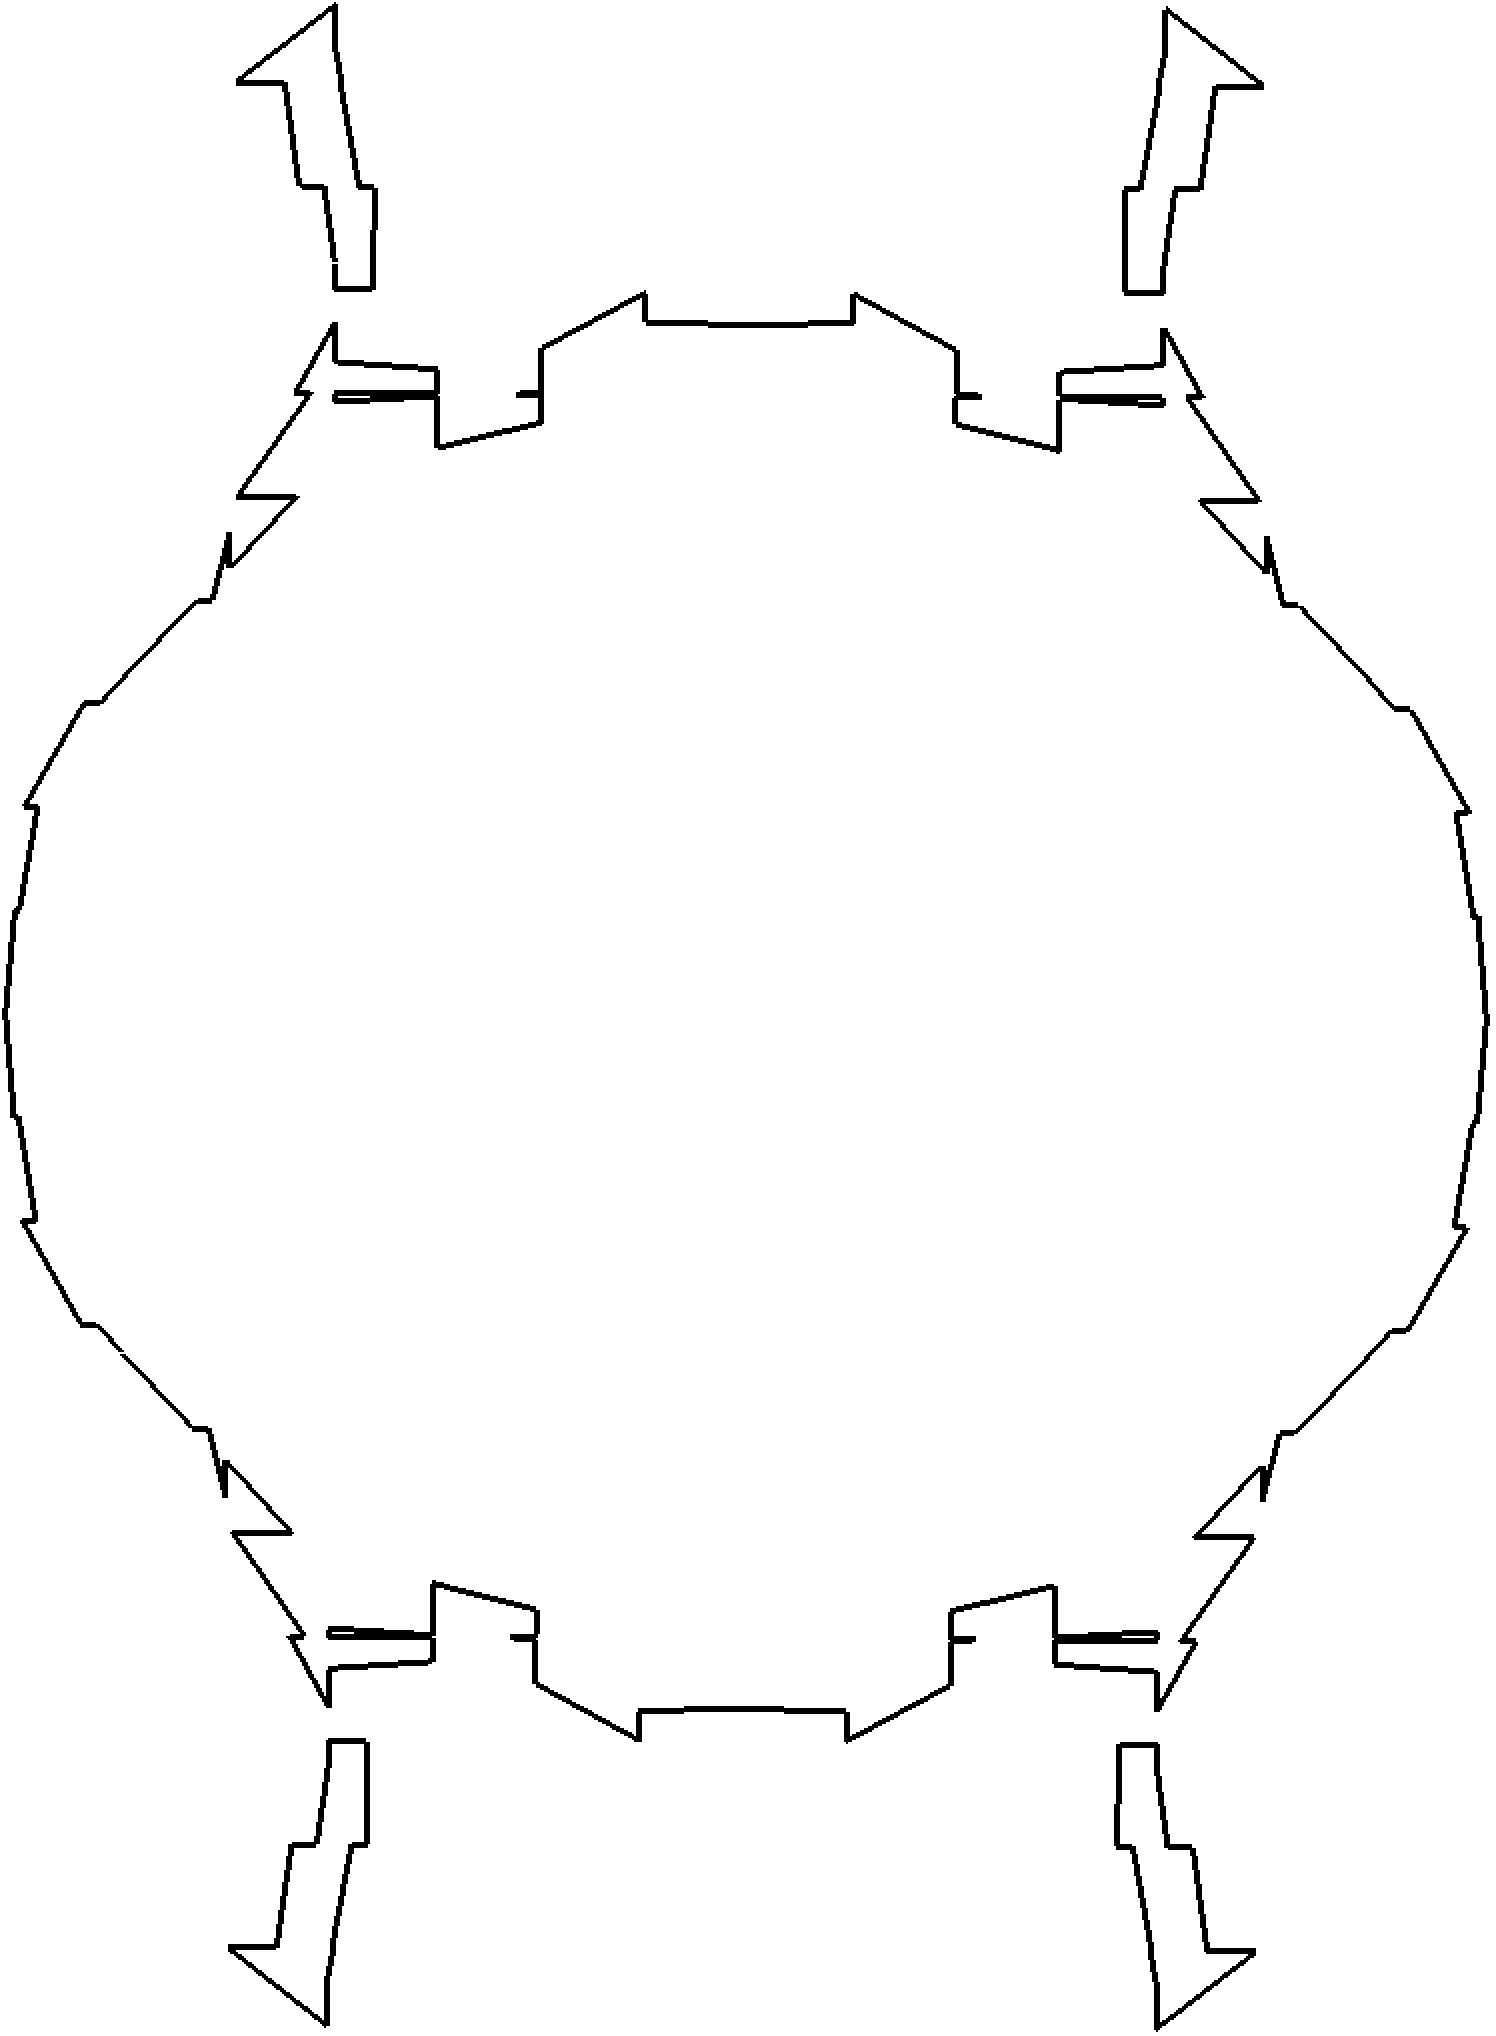
\includegraphics[scale=0.25]{figs/bad.png}
	\caption{Standard method interface breakup.}
	\label{bad2} 
\end{figure} 
